\documentclass{beamer}
\usepackage[version=4]{mhchem} 
\usepackage{tikz}


\usetheme{Madrid}
\usecolortheme{beaver}

\title{Unit 2}
\subtitle{Waves}
\author{Mr. Maxwell}
\institute{PACS}
\date{\today}


\begin{document}

\frame{\titlepage}
\frame{\tableofcontents}

\section{Wave Vocabulary}

\subsection{Wave Types}

\subsubsection{mechanical waves}

\begin{frame}
    \frametitle{mechanical waves}
    
    \begin{enumerate}
        \item require a medium, or material(i.e. gas, liquid, solid), for transmission
        \item energy comes from a vibrating source
        \item the wave passes through a medium, but the medium itself does not travel along with the wave as energy is transmitted.
    \end{enumerate}
\end{frame}

\subsubsection{electromagnetic waves}

\begin{frame}
    \frametitle{electromagnetic waves}
    
    \begin{enumerate}
        \item do not need a medium
        \item include visible light as well as infrared and ultraviolet light, microwaves, X-rays, and gamma rays.
        \item  These waves are generated by oscillations of electrical and magnetic fields from charged particles
        \item  All electromagnetic waves in a vacuum move at the same speed. This speed, 3 × 108 m/s, is known as the speed of light and is represented by the letter c.
    \end{enumerate}
\end{frame}

\subsection{Wave Properties}

\subsubsection{amplitude}

\begin{frame}
    \frametitle{amplitude}
    \pause The distance from a midline to a crest or trough
    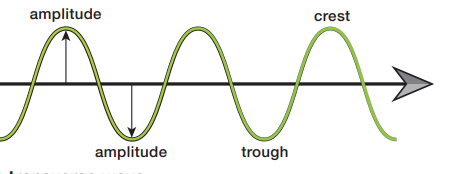
\includegraphics[width=9cm]{../../../../public/amplitude.png}
\end{frame}

\subsubsection{wavelength}

\begin{frame}
    \frametitle{wavelength}
    \pause The distance from one crest or trough to the next
    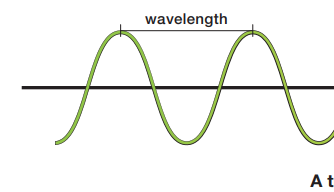
\includegraphics[width=9cm]{../../../../public/wavelength.png}
\end{frame}

\subsubsection{frequency}

\begin{frame}
    \frametitle{wavelength}
    \pause  The number of wavelengths that pass a point in a given amount of time (usually one second) is the wave's frequency(f)
    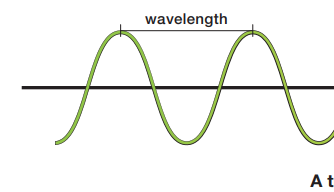
\includegraphics[width=9cm]{../../../../public/wavelength.png}
\end{frame}




\subsubsection{velocity}

\end{document}